\documentclass[14pt,a4paper,oneside]{extbook}
\usepackage[utf8]{vietnam}
\usepackage{amsmath,amssymb,mathrsfs,fancyhdr,enumerate,multirow,makecell}
\usepackage{tkz-euclide,tikz-3dplot,tikz,tkz-tab}
\usetikzlibrary{arrows.meta,calc,intersections,angles,quotes,backgrounds,shapes.geometric,patterns,through,shadows,positioning}
\usepackage{yhmath}
\usepackage[top=0.7cm, bottom=0.7cm, left=1.0cm, right=1.0cm, headheight=16pt, headsep=3mm, footskip=5mm]{geometry}
\usepackage[hidelinks,unicode]{hyperref}
\usepackage{qrcode}
\usepackage[many]{tcolorbox}
\usepackage{fontawesome}

\pagestyle{fancy}
\fancyhf{}
\fancyhead[L]{\footnotesize\bfseries\color{teal!85!black}\faBook~SỔ TAY KIẾN THỨC TOÁN 5}
\fancyhead[R]{\footnotesize\bfseries\color{blue!85!black}Lớp Toán Thầy Lĩnh -- loptoanthaylinh.vn}
\fancyfoot[C]{\footnotesize\bfseries\color{gray!80!black}-- Sổ tay kiến thức: Bài 45. Thể tích của một hình --}
\renewcommand{\headrulewidth}{0.4pt}

\begin{document}

% --- BANNER TIÊU ĐỀ BÀI HỌC ---
\noindent
\begin{tcolorbox}[
  enhanced,
  colback=teal!8!white,
  colframe=teal!80!black,
  arc=3mm,
  boxrule=1.1pt,
  width=\linewidth,
  halign=center,
  top=2.2mm, bottom=2.2mm,
  left=3mm, right=3mm,
  drop fuzzy shadow
]
  {\large\bfseries\color{teal!95!black}\faBookmark\ BÀI 45. THỂ TÍCH CỦA MỘT HÌNH}\\[2pt]
  {\scriptsize\color{black!75}\itshape Khái niệm không gian chiếm chỗ, so sánh thể tích và tính chất cộng chia thể tích trên 1 trang A4}
\end{tcolorbox}

\vspace{3.2mm}
% --- KHỐI 1: KHÁI NIỆM THỂ TÍCH ---
\noindent
\begin{minipage}[t]{0.56\textwidth}
  \begin{tcolorbox}[
    enhanced,
    title={\footnotesize\bfseries\color{white}\faCube\ 1. Khái niệm Thể tích của một hình},
    colback=blue!2!white,
    colframe=blue!75!black,
    arc=2.5mm, boxrule=0.8pt, top=1.8mm, bottom=1.8mm, left=2.2mm, right=2.2mm
  ]
    \footnotesize
    $\bullet$ Mọi vật thể trong không gian đều chiếm một khoảng không gian nhất định. Khoảng không gian đó gọi là \textbf{thể tích} của vật thể.\\
    $\bullet$ \textbf{So sánh thể tích hai hình:}\\
    $\triangleright$ \textbf{Hình này nằm trọn trong hình kia}: Hình nằm hoàn toàn bên trong có thể tích bé hơn hình bao ngoài.\\
    $\triangleright$ \textbf{Hai hình có thể tích bằng nhau}: Khi chúng được ghép bởi cùng số lượng hình lập phương nhỏ như nhau (dù hình dạng khác nhau).
  \end{tcolorbox}
\end{minipage}%
\hfill
\begin{minipage}[t]{0.42\textwidth}
  \begin{tcolorbox}[
    enhanced,
    title={\footnotesize\bfseries\color{white}\faEye\ Minh họa thể tích},
    colback=teal!2!white,
    colframe=teal!75!black,
    arc=2.5mm, boxrule=0.8pt, top=1.8mm, bottom=1.8mm, left=1.5mm, right=1.5mm,
    halign=center
  ]
    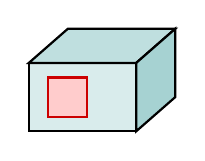
\begin{tikzpicture}[scale=0.62]
      % Hình hộp chữ nhật
      \draw[thick, fill=teal!15] (0,0) rectangle (2.2, 1.4);
      \draw[thick, fill=teal!25] (0,1.4) -- (0.8,2.1) -- (3,2.1) -- (2.2,1.4) -- cycle;
      \draw[thick, fill=teal!35] (2.2,0) -- (3,0.7) -- (3,2.1) -- (2.2,1.4) -- cycle;
      % Hình lập phương nhỏ bên trong
      \draw[red!80!black, thick, fill=red!20] (0.4,0.3) rectangle (1.2,1.1);
    \end{tikzpicture}\\[2pt]
    {\tiny\color{teal!95!black}\bfseries Khối đỏ nằm trong khối xanh $\rightarrow$ Thể tích bé hơn}
  \end{tcolorbox}
\end{minipage}

\vspace{3mm}

% --- KHỐI 2: TÍNH CHẤT BẢO TOÀN THỂ TÍCH ---
\noindent
\begin{tcolorbox}[
  enhanced,
  title={\footnotesize\bfseries\color{white}\faPuzzlePiece\ 2. Tính chất cộng và tách ghép thể tích},
  colback=purple!2!white,
  colframe=purple!70!black,
  arc=2.5mm, boxrule=0.8pt, top=1.8mm, bottom=1.8mm, left=2.5mm, right=2.5mm
]
  \footnotesize
  $\bullet$ \textbf{Tính chất ghép hình:} Khi ghép hình $A$ và hình $B$ thành hình $C$ (không đè lên nhau) thì: $\text{Thể tích hình } C = \text{Thể tích } A + \text{Thể tích } B$.\\
  $\bullet$ \textbf{Tính chất tách hình:} Khi tách một khối lớn thành các khối nhỏ, tổng thể tích các khối nhỏ bằng thể tích khối lớn ban đầu.\\
  $\bullet$ \textbf{Bảo toàn thể tích:} Uống hết nước từ chai rót sang cốc thì thể tích nước không đổi (dù hình dạng cốc khác chai).
\end{tcolorbox}

\vspace{3mm}

% --- KHỐI 3: SƠ ĐỒ TƯ DUY ---
\noindent
\begin{tcolorbox}[
  enhanced,
  title={\footnotesize\bfseries\color{white}\faSitemap\ Sơ đồ tư duy: Nhận biết \& So sánh Thể tích},
  colback=yellow!2!white,
  colframe=teal!85!black,
  arc=3mm, boxrule=0.9pt, top=1.8mm, bottom=1.8mm, left=1.5mm, right=1.5mm,
  halign=center
]
  \begin{tikzpicture}[
    scale=0.92,
    every node/.style={transform shape},
    b1/.style={rectangle, rounded corners=4pt, fill=blue!15, draw=blue!70!black, text=blue!90!black, font=\bfseries\scriptsize, inner sep=4pt, align=center},
    b2/.style={rectangle, rounded corners=4pt, fill=teal!15, draw=teal!70!black, text=teal!90!black, font=\bfseries\scriptsize, inner sep=4pt, align=center},
    b3/.style={rectangle, rounded corners=4pt, fill=green!15, draw=green!70!black, text=green!90!black, font=\bfseries\scriptsize, inner sep=4pt, align=center}
  ]
    \node[b1] (n1) at (-5.8, 0) {Định nghĩa: Khoảng\\không gian chiếm chỗ};
    \node[b2] (n2) at (0, 0) {So sánh: Đếm số khối\\lập phương đơn vị};
    \node[b3] (n3) at (5.8, 0) {Bảo toàn thể tích khi\\tách, ghép khối hình};

    \draw[teal!85!black, thick, -{Stealth[length=2.5mm]}] (n1) -- (n2);
    \draw[teal!85!black, thick, -{Stealth[length=2.5mm]}] (n2) -- (n3);
  \end{tikzpicture}
\end{tcolorbox}

\vspace{3mm}

% --- KHỐI 4: KỸ THUẬT ĐẾM KHỐI LẬP PHƯƠNG & BẪY TRẮC NGHIỆM ---
\noindent
\begin{minipage}[t]{0.54\textwidth}
  \begin{tcolorbox}[
    enhanced,
    title={\footnotesize\bfseries\color{white}\faCubes\ Kỹ thuật đếm khối lập phương theo lớp},
    colback=green!3!white,
    colframe=green!60!black,
    arc=2.5mm, boxrule=0.8pt, top=1.8mm, bottom=1.8mm, left=2.2mm, right=2.2mm
  ]
    \footnotesize
    Để không đếm sót các khối lập phương bị che khuất:\\
    $\bullet$ Đếm theo từng \textbf{lớp từ dưới lên trên} (hoặc từ trước ra sau).\\
    $\bullet$ Lớp dưới cùng có bao nhiêu khối? Lớp tiếp theo có bao nhiêu khối? Rồi cộng lại.\\
    \textit{VD:} Khối hộp $3 \times 2 \times 2$ gồm $2$ lớp, mỗi lớp $6$ khối $\rightarrow$ có $12$ khối.
  \end{tcolorbox}
\end{minipage}%
\hfill
\begin{minipage}[t]{0.44\textwidth}
  \begin{tcolorbox}[
    enhanced,
    title={\footnotesize\bfseries\color{white}\faExclamationTriangle\ Mẹo tránh bẫy trắc nghiệm},
    colback=red!2!white,
    colframe=red!70!black,
    arc=2.5mm, boxrule=0.8pt, top=1.8mm, bottom=1.8mm, left=2.2mm, right=2.2mm
  ]
    \footnotesize
    $\bullet$ \textbf{Lỗi quên khối bị che}: Khi nhìn hình vẽ 3D trên mặt giấy phẳng, học sinh hay quên đếm các khối lập phương ở phía sau hoặc ở tầng dưới cùng bị che khuất.\\
    $\bullet$ Hai hình có hình dạng hoàn toàn khác nhau vẫn có thể có thể tích bằng nhau.
  \end{tcolorbox}
\end{minipage}

\end{document}
